\documentclass[a4paper,openright]{report}
% Tipo di documento. L'uso di twoside implica che i capitoli inizino sempre con la prima pagina a sinistra, eventualmente lasciando una pagina vuota nel capitolo precedente. Se questa cosa è fastidiosa, è possibile rimuoverlo. 

% Dimensione dei margini
\usepackage[a4paper,top=3cm,bottom=3cm,left=3cm,right=3cm]{geometry} 
% Dimensione del font
\usepackage[fontsize=12pt]{scrextend}
% Lingua del testo
\usepackage[italian]{babel}
% Lingua per la bibliografia
% \usepackage[fixlanguage]{babelbib}
% Codifica del testo
\usepackage[utf8]{inputenc} 
% Font mono (quello di default non supporta il grassetto)
\usepackage{courier}
% Encoding del testo
\usepackage[T1]{fontenc}
% Permette di generare testo fittizio. Mi è stato utile 
% per capire quale sarebbe stata l'impostazione del 
% testo nella pagina prima che scrivessi un determinato paragrafo
\usepackage{lipsum}

\usepackage[
backend=biber,
bibstyle=other/custom-numeric,
citestyle=numeric,
sorting=none,
]{biblatex}
% Sorgente della bibliografia
\addbibresource{chapters/Bibliografia.bib}

% Citazioni

% Per ruotare le immagini
\usepackage{rotating}
% Per cambiare i capitoli
\usepackage{titlesec}
\titleformat{\chapter}[display]
  {\normalfont\bfseries}{}{-100pt}{\huge}
% Per mostrare nell'indice anche le subsubsection
\setcounter{tocdepth}{3}
% Per modificare l'header delle pagine 
\usepackage{fancyhdr}               

% Librerie matematiche
\usepackage{amssymb}
\usepackage{amsmath}
\usepackage{amsthm}         

% Uso delle immagini
\usepackage{graphicx}
% Uso dei colori
\usepackage[dvipsnames,svgnames,x11names]{xcolor}
% Uso dei listing per il codice
\usepackage{listings}          
% Per inserire gli hyperlinks tra i vari elementi del testo 
% \usepackage[hang, flushmargin]{footmisc}
% Diversi tipi di sottolineature
\usepackage[normalem]{ulem}

\usepackage{lstautogobble}  % Fix relative indenting
\usepackage{color}          % Code coloring
\usepackage{zi4}            % Nice font

%Aggiunti io?
\usepackage{lmodern}
\usepackage{ragged2e}
\usepackage{caption}
\usepackage[newfloat,outputdir=out]{minted}
\usepackage{float}
\usepackage[skip=5pt]{parskip}
\usepackage{setspace}
\usepackage{hyphsubst}
\usepackage{microtype}
\usepackage{hyperref}
\usepackage{footnotebackref}

% dopo minted
\usepackage{csquotes}


% Modifica lo stile dell'header
\pagestyle{fancy}
\fancyhf{}
% \fancyhead[CE,CO]{\rightmark}
% \fancyhead[LE,RO]{\textbf{\thepage}}
\fancyhead[L]{\rightmark}
\fancyhead[R]{\textbf{\thepage}}
\fancyfoot{}
\setlength{\headheight}{17pt}

% Rimuove il numero di pagina all'inizio dei capitoli
\fancypagestyle{plain}{
  \fancyfoot{}
  \fancyhead{}
  \renewcommand{\headrulewidth}{0pt}
}

% Togliendo il commento al comando che segue, si inseriscono nella bibliografia anche le fonti presenti in Bibliography.bib ma non citati direttamente con il comando \cite

% Modifica dello stile dei riferimenti, con il testo in cyano
\definecolor{DarkGreen}{RGB}{20,80,40}
\definecolor{Unipi}{RGB}{00,85,143} 
\definecolor{term_bg_color}{RGB}{240,241,240} 
\hypersetup{
    colorlinks,
    linkcolor=Unipi,
    citecolor=Unipi,
    urlcolor=Unipi
}


\DeclareCiteCommand{\supercite}[\mkbibsuperscript]
  {\iffieldundef{prenote}
     {}
     {\BibliographyWarning{Ignoring prenote argument}}%
   \iffieldundef{postnote}
     {}
     {\BibliographyWarning{Ignoring postnote argument}}}
  {\usebibmacro{citeindex}%
   \bibopenbracket\usebibmacro{cite}\bibclosebracket}
  {\supercitedelim}
  {}


% Aggiunti definizioni, teoremi, linea e listing
\newtheorem{definition}{Definizione}[section]
\newtheorem{theorem}{Teorema}[section]
\providecommand*\definitionautorefname{Definizione}
\providecommand*\theoremautorefname{Teorema}
\providecommand*{\listingautorefname}{Listing}
\providecommand*\lstnumberautorefname{Linea}

\raggedbottom

\usepackage{tcolorbox}
\usepackage{xpatch}


% -----------------------------------------------------------------

\begin{document}

\setlength{\fboxsep}{0pt}
\selectlanguage{italian}

% \hyphenpenalty=10000
% \exhyphenpenalty=10000

% \loadspellchecklist[it][wordlist.txt]
% \setupspellchecking[state=start]

% \setminted{
    linenos=true,
    numbersep=5pt,
    bgcolor=term_bg_color,
    frame=single,
    framesep=5pt,
    tabsize=2,
    breaklines=true,
    baselinestretch=0.9
}

\setlength{\abovecaptionskip}{-2pt} 
\setlength{\belowcaptionskip}{8pt} 

\newenvironment{code}
    {\captionsetup{type=listing}}
    {\par\noindent\ignorespacesafterend}

\SetupFloatingEnvironment{listing}{name=Listing, listname=List of Listings}

\usemintedstyle{sas}
% \usemintedstyle{unipi}
% \usemintedstyle{xcode}
% \usemintedstyle[output]{rrt}

% Interlinea
\setstretch{1.1}

\begin{titlepage}
\begin{figure}[!htb]

\begin{center}
{
    
\includegraphics[keepaspectratio=true,scale=0.5]{images/Frontespizio/cherubinFrontespizio.eps}
}
\end{center}

\end{figure}

\begin{center}
    \LARGE{UNIVERSITÀ DI PISA}
\end{center}

\vspace{15mm}
\begin{center}
    {\LARGE{\bf CORDIC: Cartesian to  \\ \vspace{3mm} Polar Coordinate Transformation }}
\end{center}
\vspace{30mm}

\vfill
\hrulefill
\\\centering{\large{ANNO ACCADEMICO 2024/2025}}

\end{titlepage}
\stepcounter{page}

\tableofcontents


\chapter{Introduction}

\section{Specification}

\section{Circuit Applications}
\chapter{Architecture}

\chapter{VHDL code}


\section{CORDIC}
The following code shows the implementation of the CORDIC in vectoring mode for cartesian to polar conversion. This implementation supports the fix step for accepting inputs in all 4 quadrants, and also normalizes \( \rho \).

\begin{code}
    \vhdlCode{../vhdl/src/CORDIC.vhd}
    \captionof{listing}{\texttt{CORDIC.vhd}}
    \label{code:vhdl}
\end{code}


\section{Atan LUT}
The values of the LUT table were calculated using the formula:
\[
    \text{LUT}_i = \left\lfloor \text{atan}(2^{-i} )* 2^{21} \right\rfloor
\]
\begin{code}
    \vhdlCode{../vhdl/src/ATAN_LUT.vhd}
    \captionof{listing}{\texttt{ATAN\_LUT.vhd}}
    \label{code:lut}
\end{code}

\chapter{Verification and testing}

\section{Testbench}



\begin{code}
    \inputminted{vhdl}{listings/04/CORDIC_tb.vhd}
    \captionof{listing}{\texttt{CORDIC\_tb.vhd}}
    \label{code:testbench}
\end{code}

\chapter{Synthesis and Implementation}

\section{Vivado Design flow}

\section{RTL}

\section{RTL Elaboration}

\section{Synthesis and Implementation}





\chapter{Vivado results}

\section{Critical Path}
\begin{figure}[H]
    \centering
    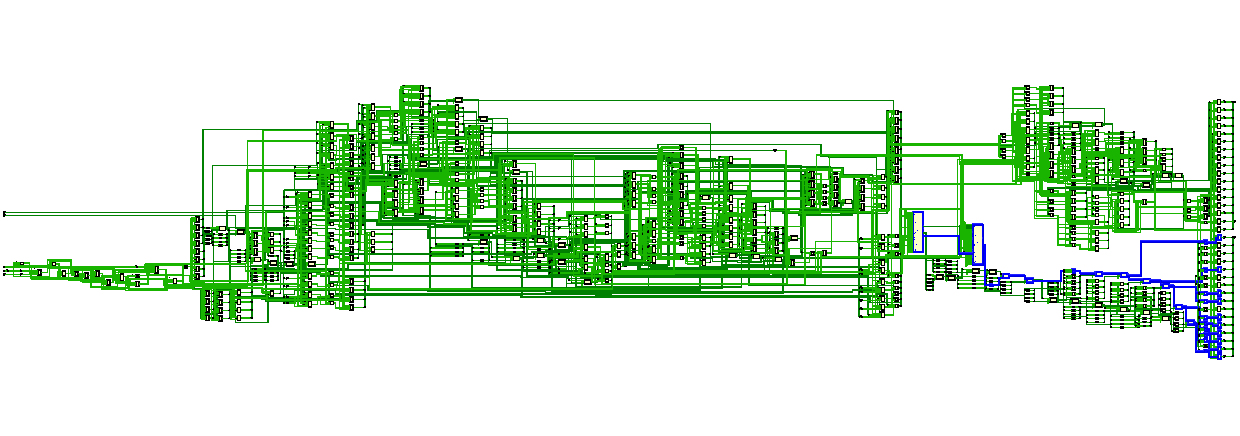
\includegraphics[width=\textwidth]{./images/Vivado/setup_synthesis.pdf}
    \caption{Figure showing the elaborated RTL design with the main critical paths for set-up-time-violation found in synthesis step highlighted in blue.}
    \label{fig:setup_synthesis}
\end{figure}

\begin{table}[ht]
    \centering
    \small
    \captionsetup{skip=10pt} 
    \begin{tabular}{lrrrrrrr}
        \hline
        Name &  Slack &  Levels &  Routes & From      & To                 & Total Delay    \\
        \hline
        Path 1 &   9.30 &      12 &       6 & ARG2/CLK  & x\_out\_reg[15]/D  &        10.55  \\
        Path 2 &   9.33 &      11 &       6 & ARG2/CLK  & x\_out\_reg[12]/D  &        10.52  \\
        Path 3 &   9.45 &      10 &       6 & ARG2/CLK  &  x\_out\_reg[8]/D  &        10.40  \\
        Path 4 &   9.51 &      12 &       6 & ARG2/CLK  & x\_out\_reg[14]/D  &        10.33  \\
        Path 5 &   9.56 &       9 &       6 & ARG2/CLK  &  x\_out\_reg[4]/D  &        10.28  \\
        Path 6 &   9.57 &      11 &       6 & ARG2/CLK  & x\_out\_reg[11]/D  &        10.28  \\
        Path 7 &   9.62 &      12 &       6 & ARG2/CLK  & x\_out\_reg[13]/D  &        10.23  \\
        Path 8 &   9.62 &      11 &       6 & ARG2/CLK  & x\_out\_reg[10]/D  &        10.23  \\
        Path 9 &   9.67 &       8 &       6 & ARG2/CLK  &  x\_out\_reg[0]/D  &        10.18  \\
        Path 10 &   9.69 &      10 &       6 & ARG2/CLK  &  x\_out\_reg[7]/D  &       10.16  \\
        \hline
    \end{tabular}
    \caption{Table showing data of the main critical paths found in synthesis step}
    \label{tab:setup_synthesis}
\end{table}
    

\begin{figure}[H]
    \centering
    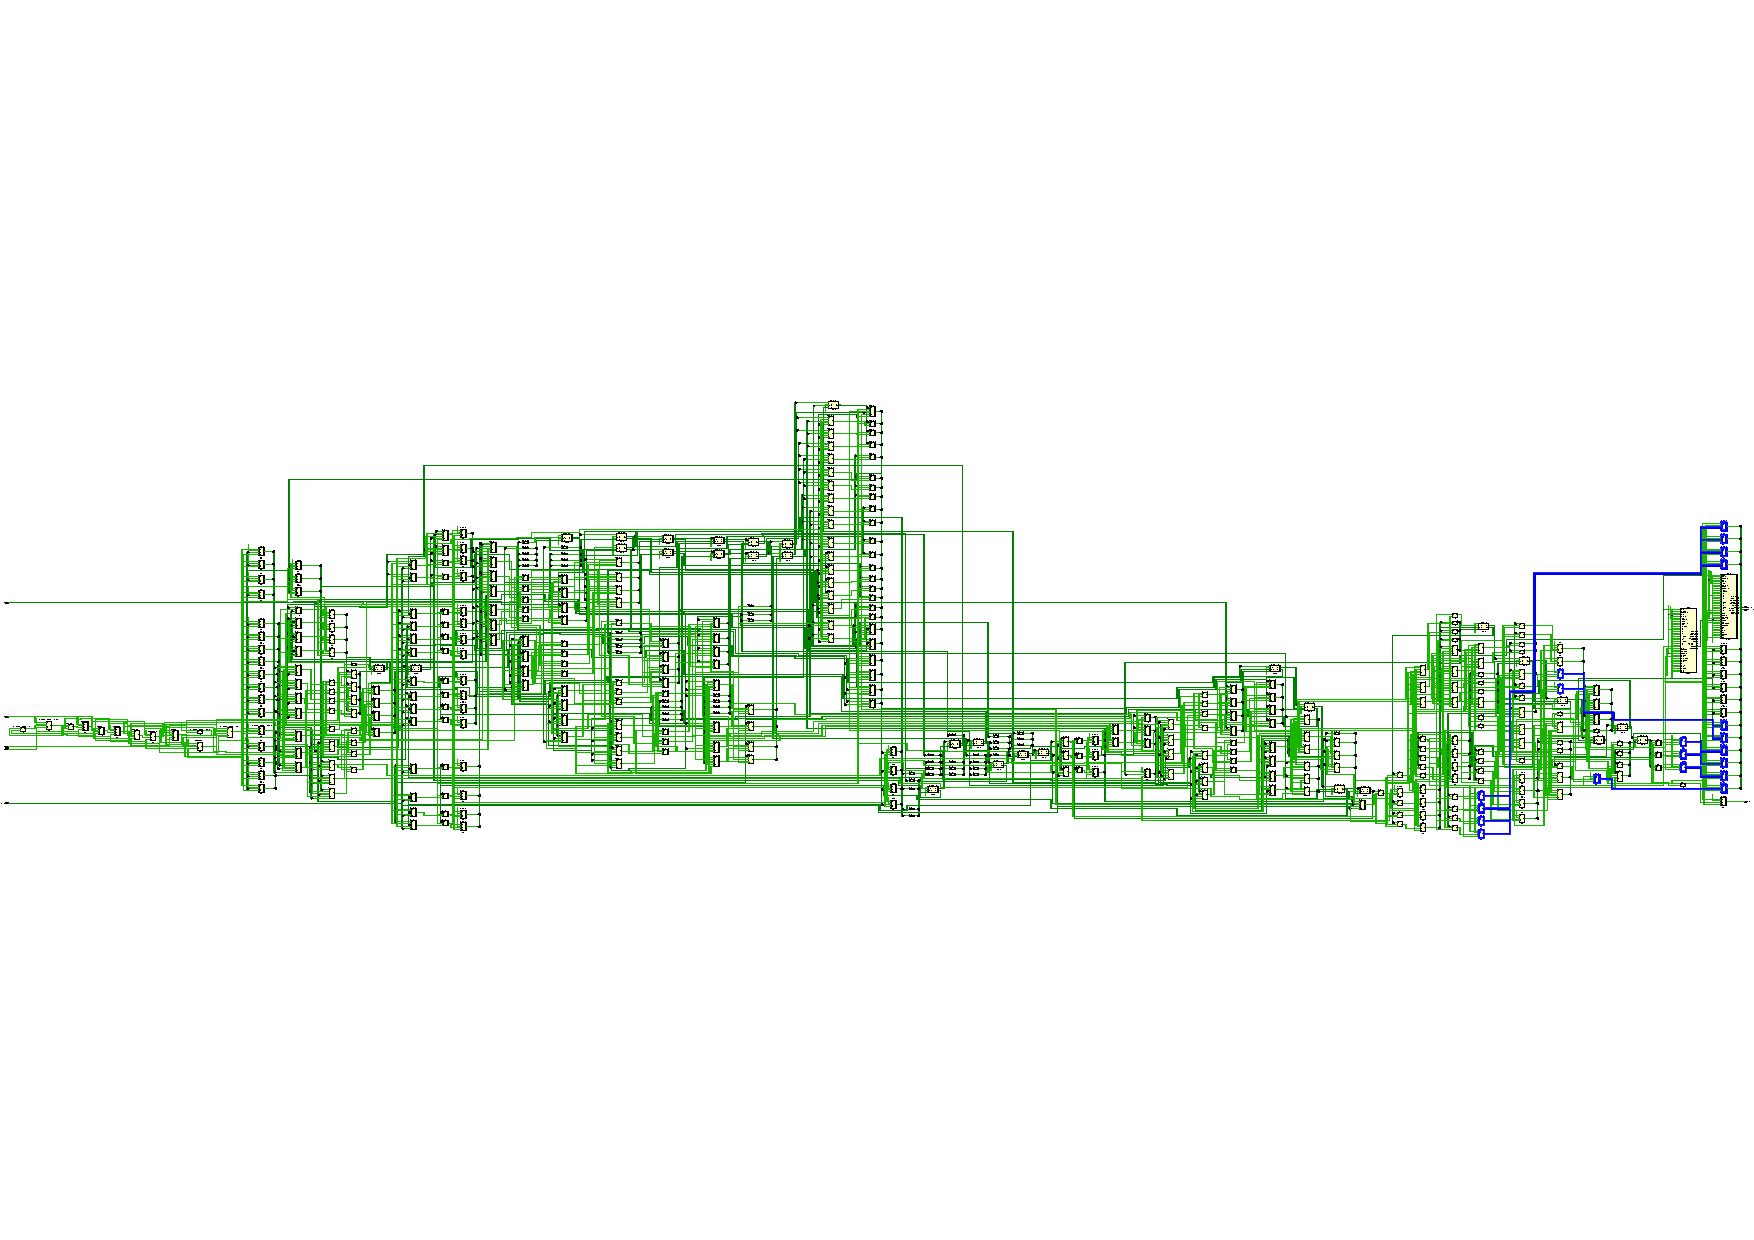
\includegraphics[width=\textwidth]{./images/Vivado/hold_synthesis.pdf}
    \caption{Figure showing the elaborated RTL design with the main critical paths for hold-time-violation found in synthesis step highlighted in blue.}
    \label{fig:hold_synthesis}
\end{figure}  

\begin{table}[ht]
    \centering
    \small
    \captionsetup{skip=10pt} 
    \begin{tabular}{lrrrrrr}
        \hline
        Name    & Slack & Levels & Routes  & From           & To               & Total Delay \\
        \hline
        Path 11 & 0.16  & 0      & 1       & z\_t\_reg[23]/C & z\_out\_reg[15]/D & 0.29       \\
        Path 12 & 0.16  & 0      & 1       & z\_t\_reg[8]/C  & z\_out\_reg[0]/D  & 0.29       \\
        Path 13 & 0.16  & 0      & 1       & z\_t\_reg[18]/C & z\_out\_reg[10]/D & 0.29       \\
        Path 14 & 0.16  & 0      & 1       & z\_t\_reg[19]/C & z\_out\_reg[11]/D & 0.29       \\
        Path 15 & 0.16  & 0      & 1       & z\_t\_reg[20]/C & z\_out\_reg[12]/D & 0.29       \\
        Path 16 & 0.16  & 0      & 1       & z\_t\_reg[21]/C & z\_out\_reg[13]/D & 0.29       \\
        Path 17 & 0.16  & 0      & 1       & z\_t\_reg[22]/C & z\_out\_reg[14]/D & 0.29       \\
        Path 18 & 0.16  & 0      & 1       & z\_t\_reg[9]/C  & z\_out\_reg[1]/D  & 0.29       \\
        Path 19 & 0.16  & 0      & 1       & z\_t\_reg[10]/C & z\_out\_reg[2]/D  & 0.29       \\
        Path 20 & 0.16  & 0      & 1       & z\_t\_reg[11]/C & z\_out\_reg[3]/D  & 0.29       \\
        \hline
    \end{tabular}
    \caption{Table showing the characteristics regarding critical paths for hold-time-violation found in synthesis step.}
    \label{tab:hold_synthesis}
\end{table}


\begin{table}[ht]
    \centering
    \small
    \captionsetup{skip=10pt} 
    \begin{tabular}{lrrrrrr}
        \hline
        Name    & Slack & Levels & Routes & From      & To                 & Total Delay \\
        \hline
        Path 1  & 8.90  & 10     & 3      & ARG2/CLK  & x\_out\_reg[9]/D   & 10.99       \\
        Path 2  & 8.93  & 10     & 3      & ARG2/CLK  & x\_out\_reg[12]/D  & 10.96       \\
        Path 3  & 8.99  & 11     & 3      & ARG2/CLK  & x\_out\_reg[13]/D  & 10.86       \\
        Path 4  & 9.08  & 11     & 3      & ARG2/CLK  & x\_out\_reg[15]/D  & 10.82       \\
        Path 5  & 9.10  & 9      & 3      & ARG2/CLK  & x\_out\_reg[8]/D   & 10.84       \\
        Path 6  & 9.10  & 9      & 3      & ARG2/CLK  & x\_out\_reg[6]/D   & 10.84       \\
        Path 7  & 9.14  & 10     & 3      & ARG2/CLK  & x\_out\_reg[10]/D  & 10.71       \\
        Path 8  & 9.15  & 9      & 3      & ARG2/CLK  & x\_out\_reg[7]/D   & 10.74       \\
        Path 9  & 9.18  & 11     & 3      & ARG2/CLK  & x\_out\_reg[14]/D  & 10.72       \\
        Path 10 & 9.22  & 10     & 3      & ARG2/CLK  & x\_out\_reg[11]/D  & 10.63       \\
        \hline
    \end{tabular}
    \caption{Table showing the main critical paths for the setup-time-violation during the implementation step.}
    \label{tab:setup_implementation}
\end{table}


\begin{table}[ht]
    \centering
    \small
    \captionsetup{skip=10pt} 
    \begin{tabular}{lrrrrrr}
        \hline
        Name    & Slack & Levels & Routes  & From                              & To                    & Total Delay \\
        \hline
        Path 11 & 0.17  & 1      & 1       & counter\_reg[0]/C                & counter\_reg[2]/D     & 0.31       \\
        Path 12 & 0.17  & 1      & 1       & counter\_reg[0]/C                & counter\_reg[1]/D     & 0.31       \\
        Path 13 & 0.18  & 1      & 1       & counter\_reg[0]/C                & counter\_reg[3]/D     & 0.31       \\
        Path 14 & 0.22  & 0      & 1       & z\_t\_reg[19]/C                  & z\_out\_reg[11]/D     & 0.25       \\
        Path 15 & 0.22  & 0      & 1       & z\_t\_reg[23]/C                  & z\_out\_reg[15]/D     & 0.27       \\
        Path 16 & 0.23  & 0      & 1       & z\_t\_reg[8]/C                   & z\_out\_reg[0]/D      & 0.26       \\
        Path 17 & 0.25  & 0      & 1       & z\_t\_reg[12]/C                  & z\_out\_reg[4]/D      & 0.35       \\
        Path 18 & 0.25  & 0      & 1       & z\_t\_reg[22]/C                  & z\_out\_reg[14]/D     & 0.33       \\
        Path 19 & 0.26  & 1      & 1       & FSM\_reg[0]/C                    & FSM\_reg[0]/D         & 0.35 \\
        Path 20 & 0.27  & 0      & 1       & z\_t\_reg[18]/C                  & z\_out\_reg[10]/D     & 0.37       \\
        \hline
    \end{tabular}
    \caption{Table showing the main critical paths for hold-time-violation found in the implementation step.}
    \label{tab:hold_implementation}
\end{table}

\cadm{need to comment a bit these results, for example the paths for setup-time-violation correspond exactly between synthesis and implementation, whereas hold-time-violation are different, these means that place and route had a significant impact in determining these values. }

\cadm{The DRC actually gives us 6 warnings, it tells us to pipeline the multiplier block in order to enhance performances and power consumption.
But we adopted a CORDIC approach with loopbacks, that converges in 16 steps, 17 in the worst case when we have the fix step, 
inserting a register in between would cause higher delays in order to get the result. }


\section{Utilization Report}
\begin{table}[ht]
    \centering
    \small
    \captionsetup{skip=10pt} 
    \begin{tabular}{lrr}
        \hline
        Resource               & Utilization (\%) & Description \\
        \hline
        Slice LUTs             & 2.05\%           & Look-Up Tables used as logic \\
        Slice Registers        & 0.32\%           & Registers used in the design \\
        Slice                  & 2.30\%           & Total slices utilized \\
        LUT as Logic           & 2.05\%           & LUTs specifically used as logic \\
        DSPs                   & 2.50\%           & Digital Signal Processing blocks \\
        Bonded IOB             & 68.00\%          & Bonded Input/Output Blocks \\
        BUFGCTRL               & 3.13\%           & Global Clock Buffers \\
        \hline
    \end{tabular}
    \caption{Resource utilization for the CORDIC design (only non-zero values shown)}
    \label{tab:cordic_resource_utilization}
\end{table}


\section{Power Report}
\begin{figure}[H]
    \centering
    \captionsetup{skip=10pt} 
    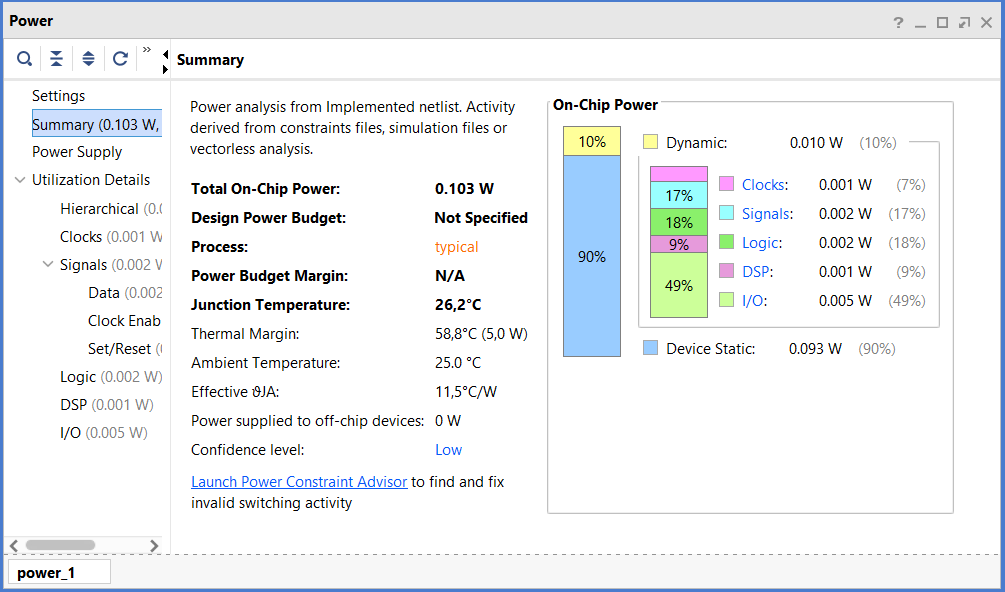
\includegraphics[width=\textwidth]{./images/Vivado/power_report.png}
    \caption{Vivado Power Report after implementation.}
    \label{fig:power_report}
\end{figure}
\chapter{Final considerations}


\nocite{*}
\printbibliography

\end{document}
% -----------------------------------------------------------------
